\documentclass{beamer}
\usepackage[utf8]{inputenc}

\usepackage{caption}
\usepackage{subcaption}
\setbeamertemplate{caption}[numbered]

\usetheme{Madrid}
\usecolortheme{default}

%path to the images
\graphicspath{{../../images/},{../../images/presentation/}}

%------------------------------------------------------------
%This block of code defines the information to appear in the
%Title page
\title[UAM Baja SAE team 2023] %optional
{Progress and requirements of the instrumentation section}
\subtitle{UAM Baja SAE team 2023}

\author[Instrumentation section] {
	\textbf{Instrumentation section:} \\
	\vspace{0.5cm}
	 Delgadillo Marín Sergio (2162000251)\\
	 Solanes Herrera Antonio (2212000043) 
}

\date[July 2023] % (optional)
{July 2023}

\logo{
\includegraphics[height=1cm]{logo.jpg}}

%End of title page configuration block
%------------------------------------------------------------


%------------------------------------------------------------
%The next block of commands puts the table of contents at the 
%beginning of each section and highlights the current section:

\AtBeginSection[]
{
	\begin{frame}
		\frametitle{Table of Contents}
		\tableofcontents[currentsection]
	\end{frame}
}
%------------------------------------------------------------

\begin{document}
	
	%The next statement creates the title page.
	\frame{\titlepage}
	
	%---------------------------------------------------------
	%This block of code is for the table of contents after
	%the title page
	\begin{frame}
		\frametitle{Table of Contents}
		\tableofcontents
	\end{frame}
	%---------------------------------------------------------
	
	
	\section{Progress}
	
	%---------------------------------------------------------
	%Changing visivility of the text
	\begin{frame}
		\frametitle{Parameters to measure}
		List of the parameters that we are considering.
		\begin{itemize}
			\item Engine and CVT temperature.
			\item Engine and CVT RPM.
			\item Position af the shock absorbers.
			\item Speed of the wheels (vehicle).
			\item Tire pressure and temperature.
			\item Steering angle.
			\item Brake pressure.
			\item Laps data logging.
			\item Localization (GPS-Data Fusion).
			\item Inertial measurement unit.
		\end{itemize}
	\end{frame}

	\begin{frame}
		A hall sensor was proposed.
		\frametitle{Test of the speed sensors}
		\begin{figure}
			\centering
			\begin{subfigure}[b]{0.3\textwidth}
				\centering
				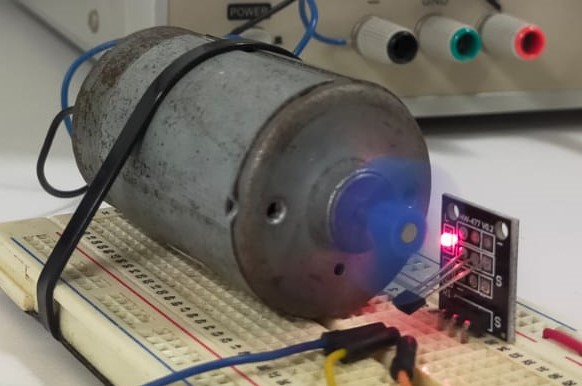
\includegraphics[width=\textwidth]{hall_1}
			\end{subfigure}
			\hfill
			\begin{subfigure}[b]{0.3\textwidth}
				\centering
				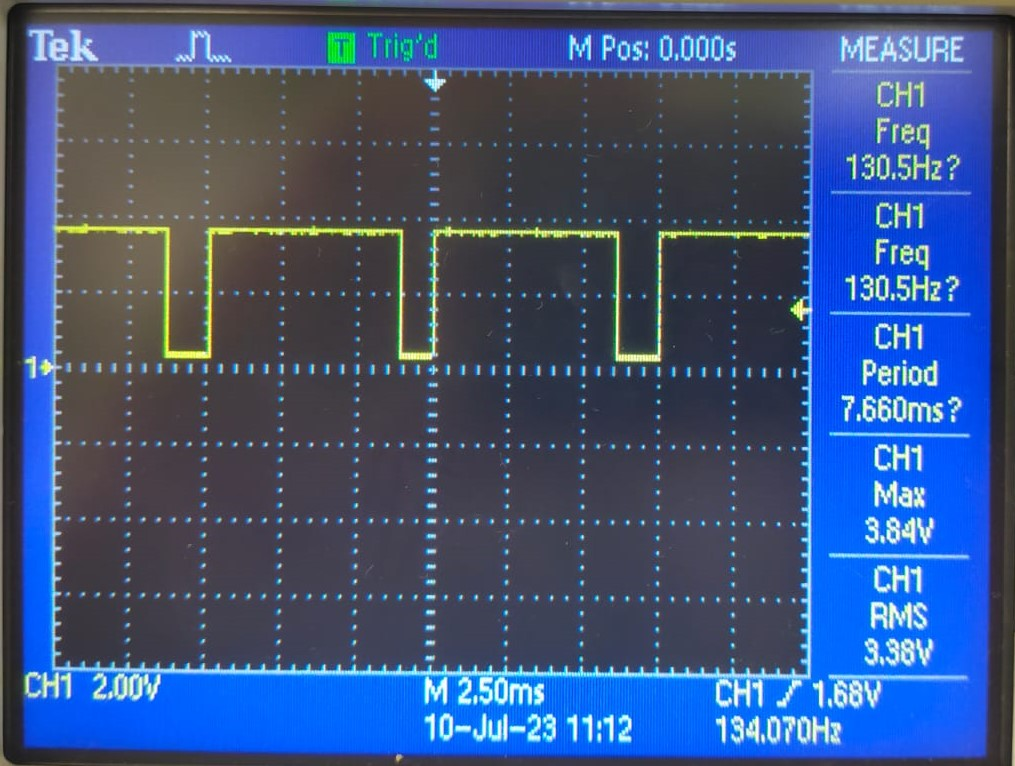
\includegraphics[width=\textwidth]{hall_2}
			\end{subfigure}
			\hfill
		\begin{subfigure}[b]{0.3\textwidth}
			\centering
			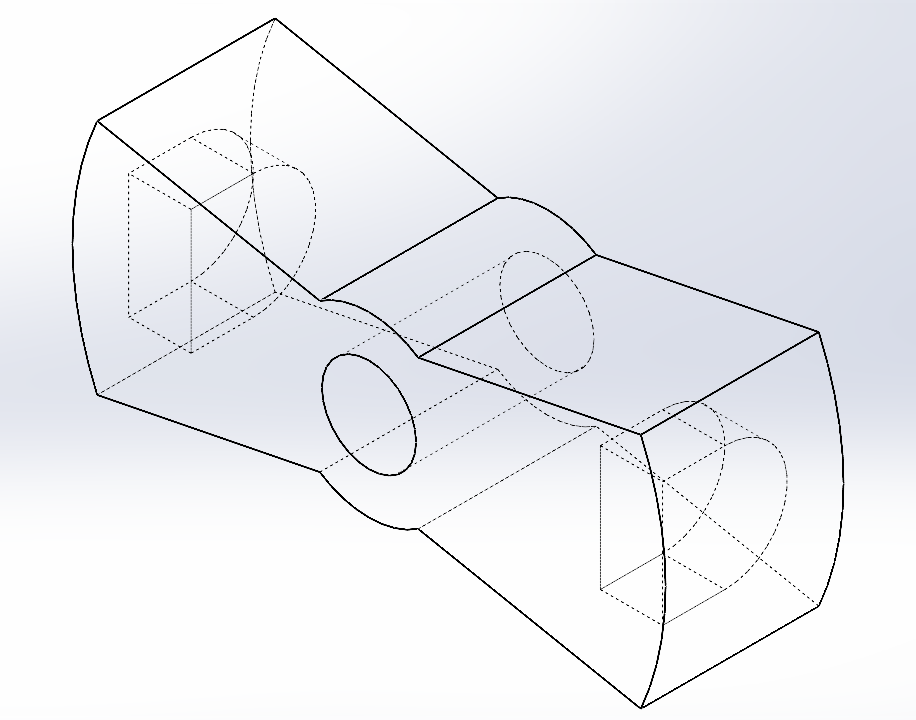
\includegraphics[width=\textwidth]{hall_3}
		\end{subfigure}
			\caption{Test of the sensor hall with a CD motor.}
			\label{fig:hall}
		\end{figure}

	\end{frame}

	\begin{frame}
		\frametitle{Collector designs}
		\begin{figure}
			\centering
			\begin{subfigure}[b]{0.3\textwidth}
				\centering
				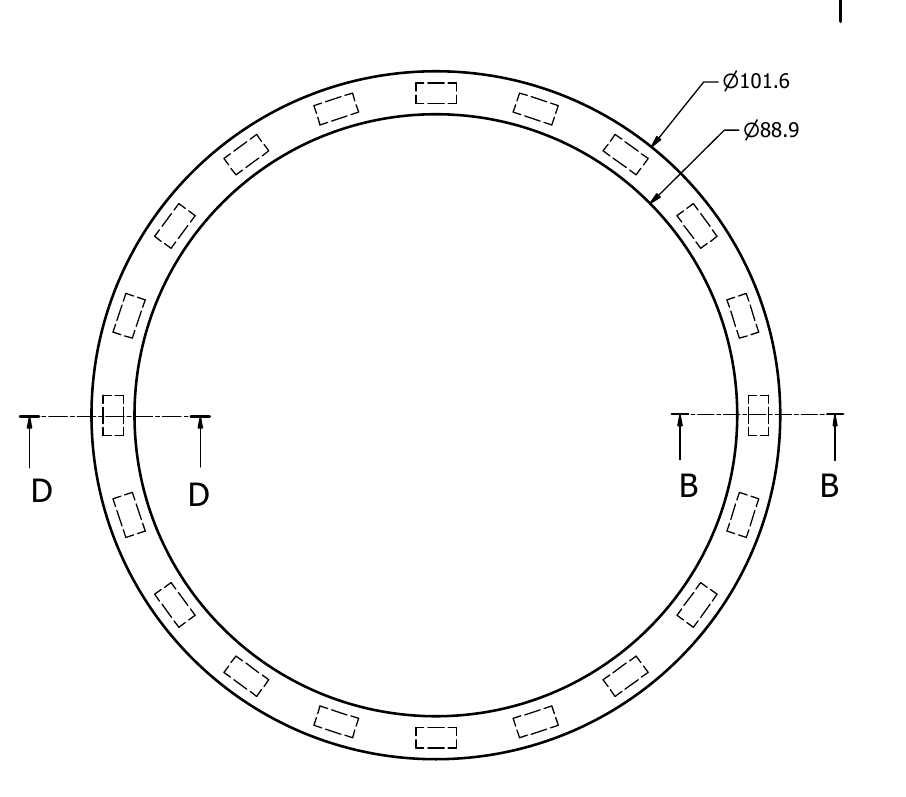
\includegraphics[width=\textwidth]{abs_ring}
			\end{subfigure}
			\hfill
			\begin{subfigure}[b]{0.3\textwidth}
				\centering
				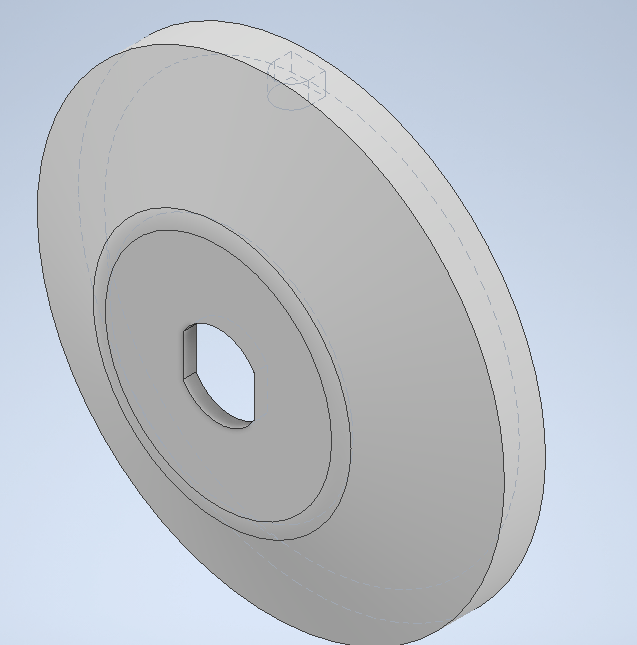
\includegraphics[width=\textwidth]{engine_ring}
			\end{subfigure}
			\hfill
			\begin{subfigure}[b]{0.3\textwidth}
				\centering
				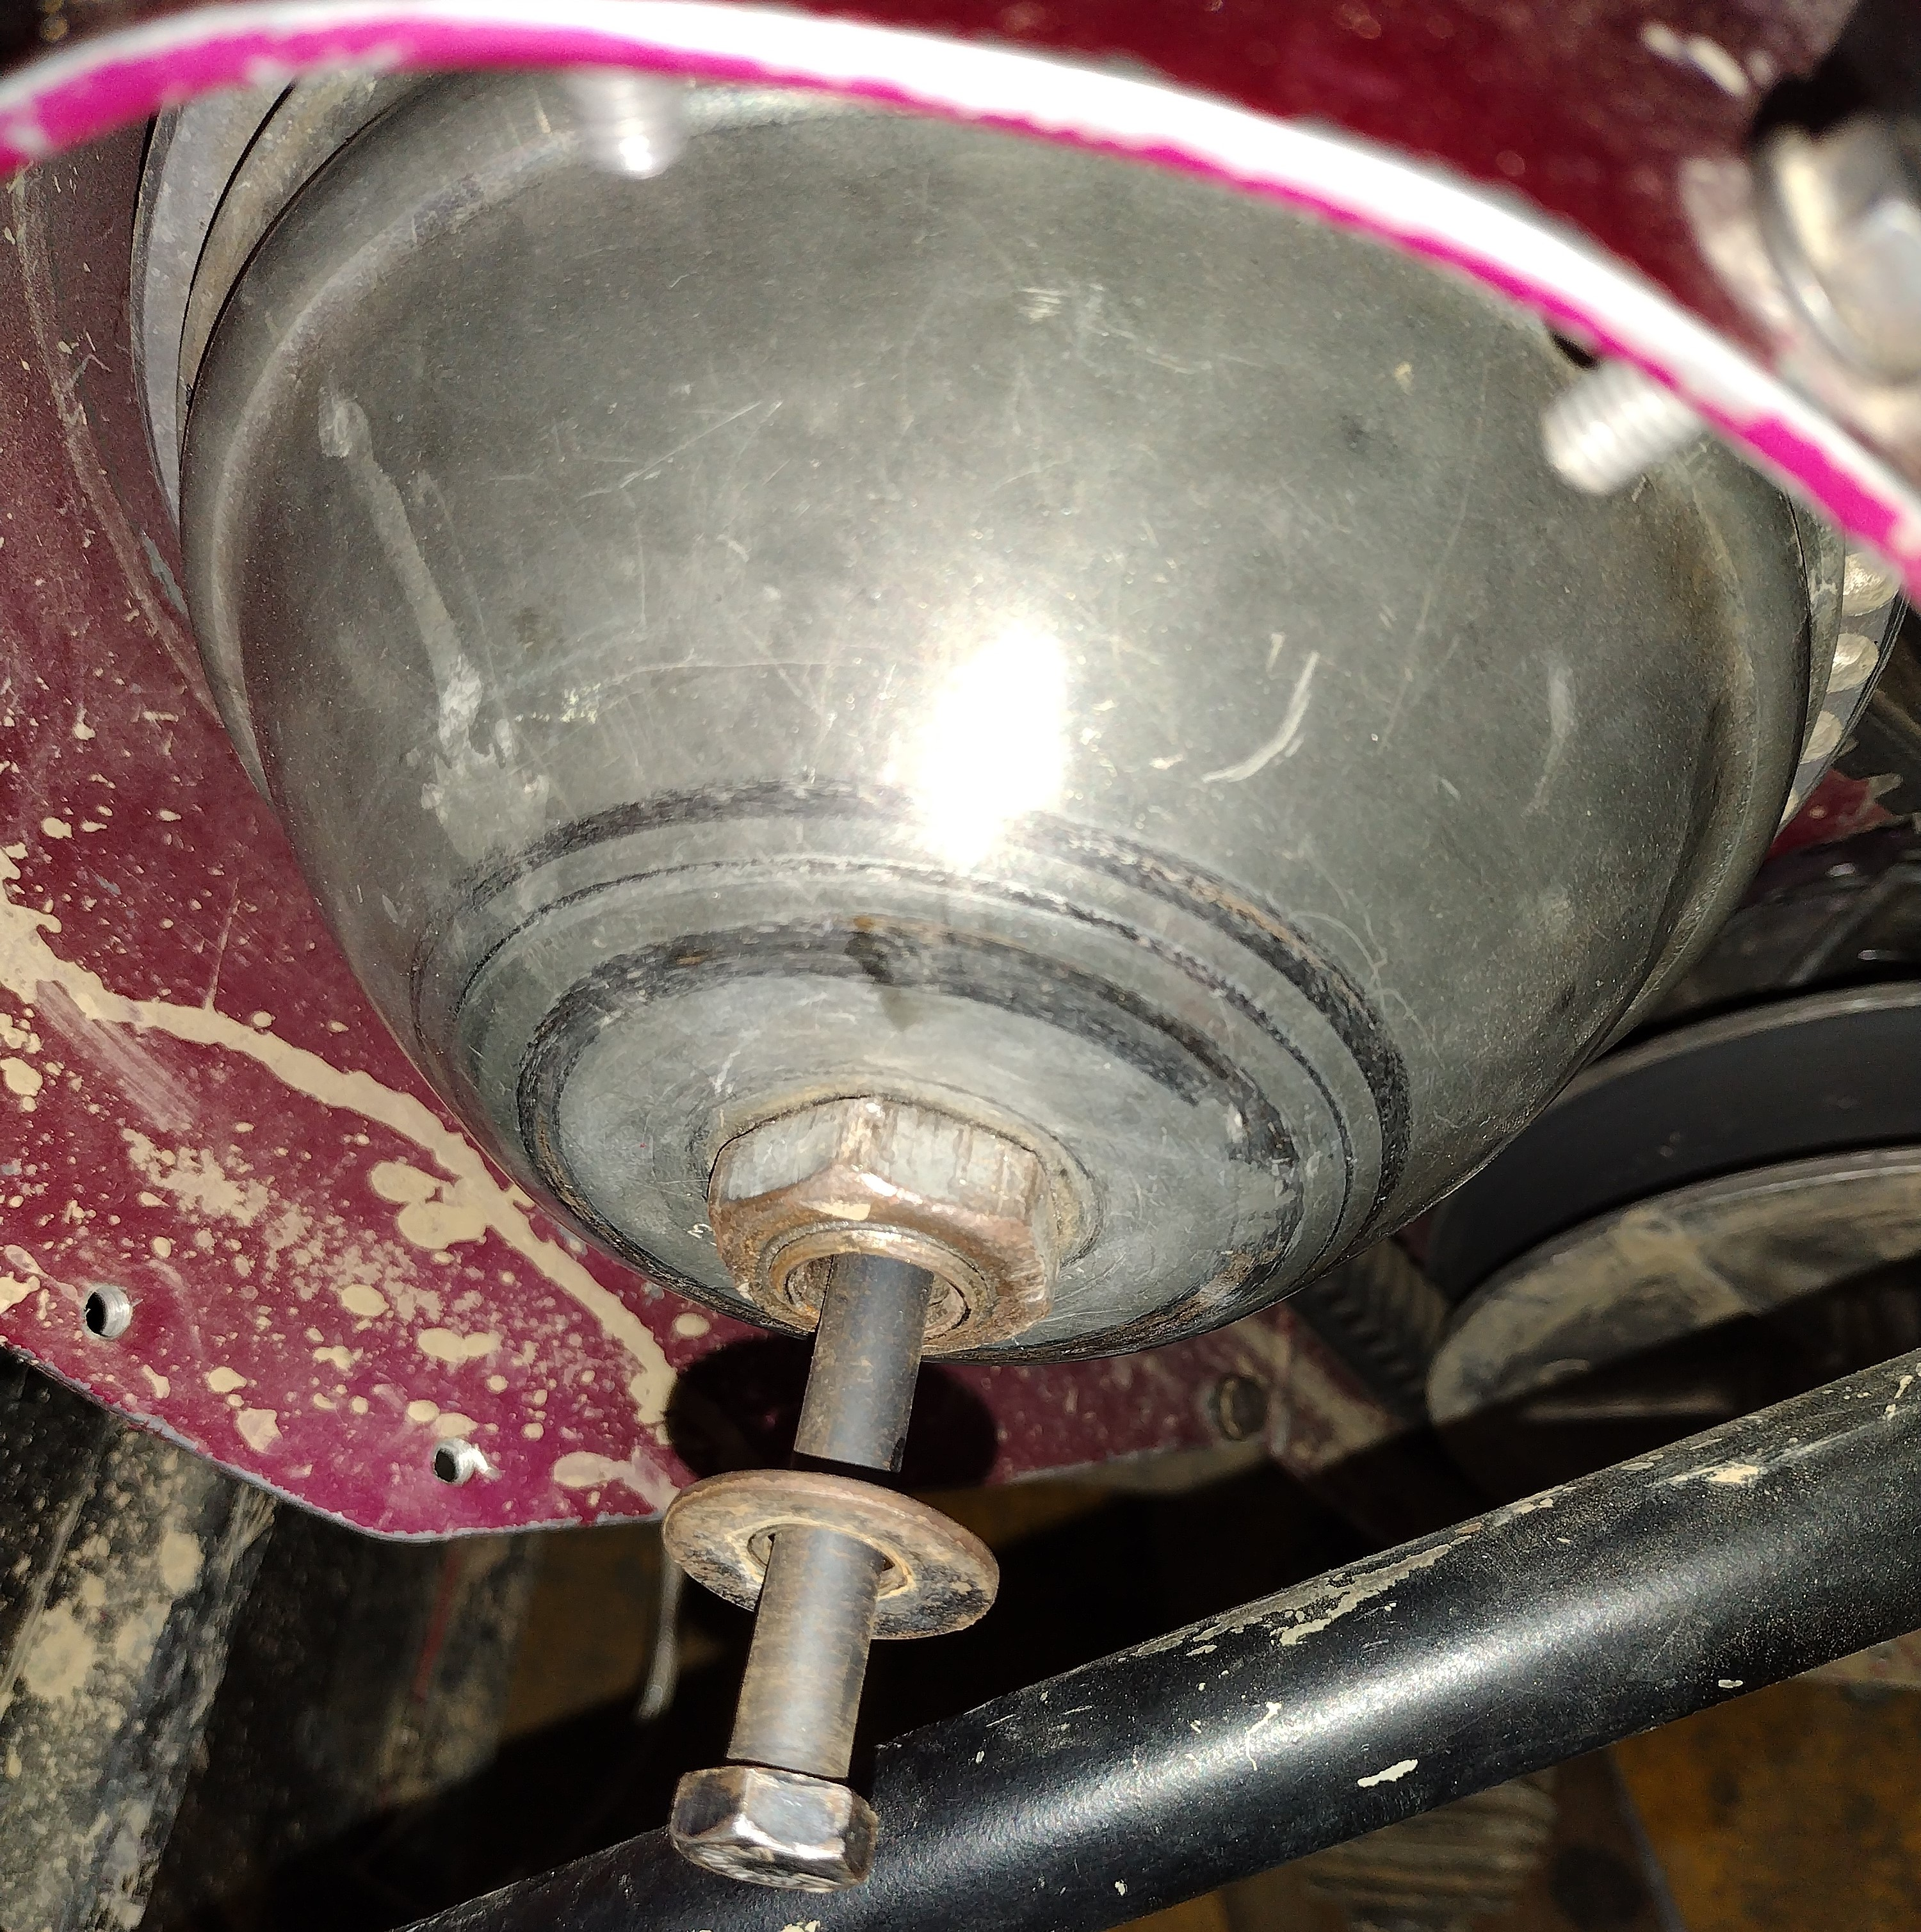
\includegraphics[width=\textwidth]{rpm_2}
			\end{subfigure}
			\caption{Prototypes of the collectors.}
			\label{fig:rings}
		\end{figure}
	\end{frame}

	\begin{frame}
		\frametitle{Communication test}
		The range obtained was of the 130m.
		\begin{figure}
			\centering
			\begin{subfigure}[b]{0.2\textwidth}
				\centering
				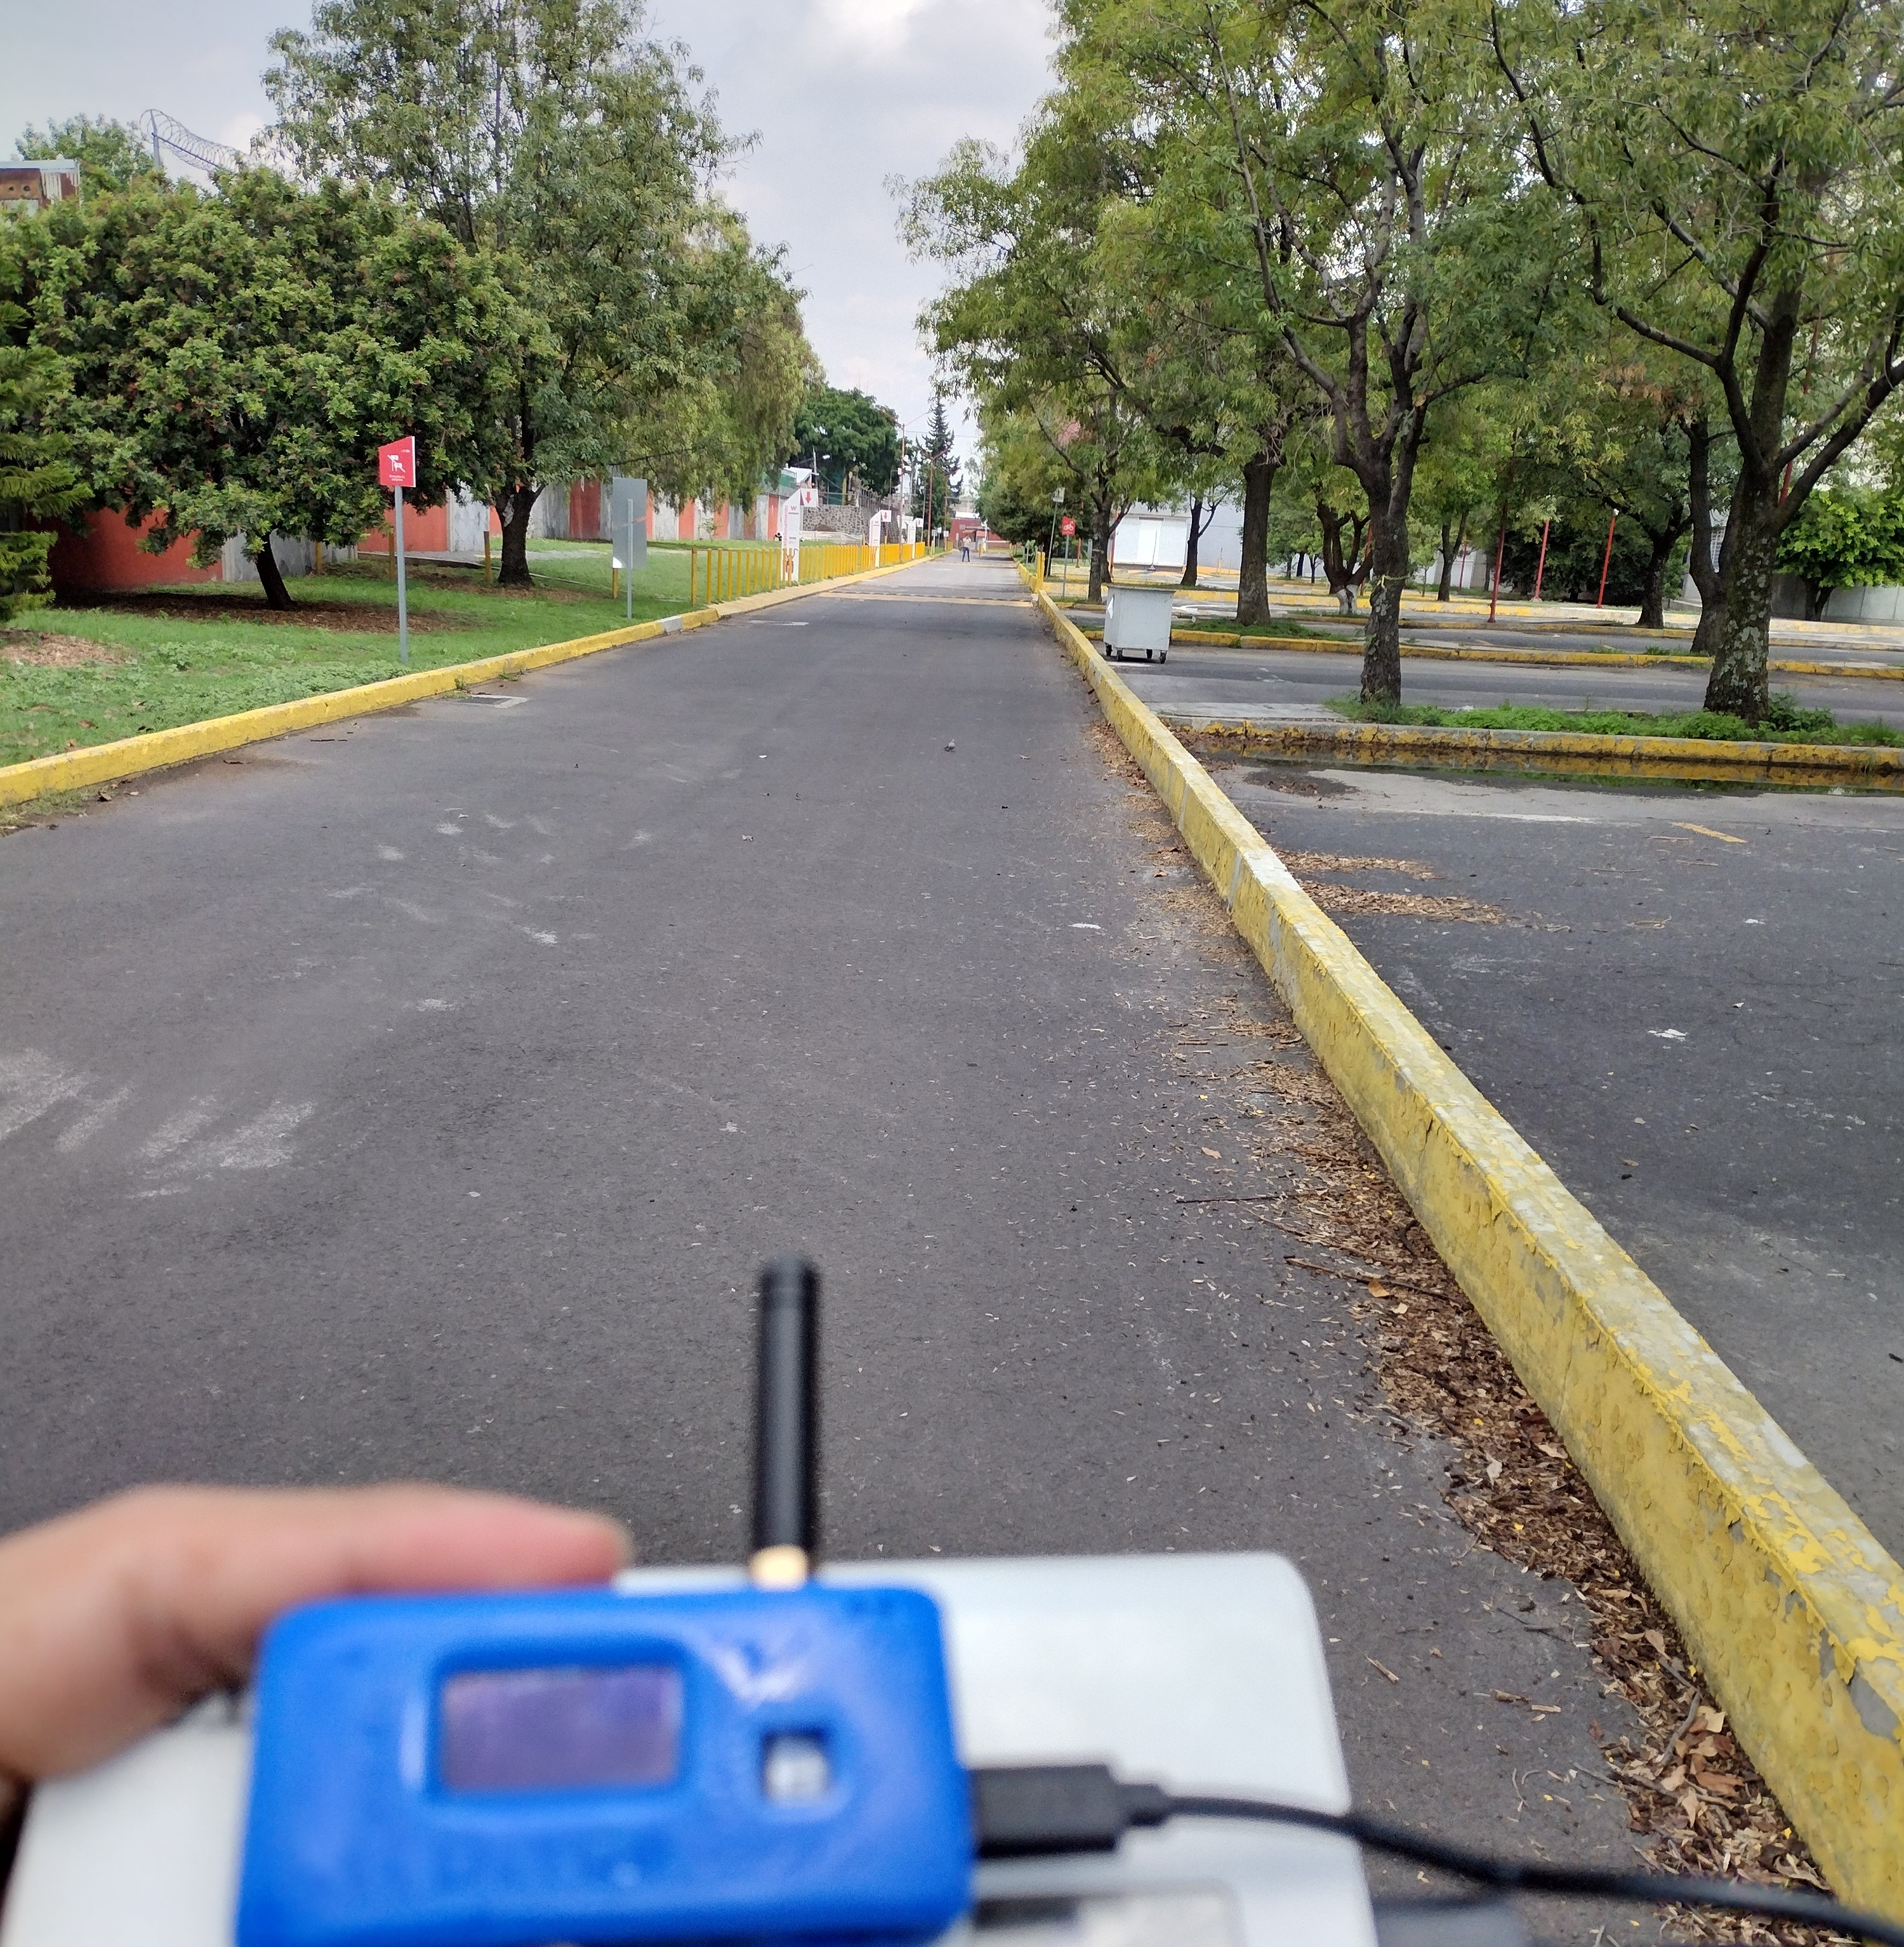
\includegraphics[width=\textwidth]{receiver_test}
			\end{subfigure}
			\hfill
			\begin{subfigure}[b]{0.7\textwidth}
				\centering
				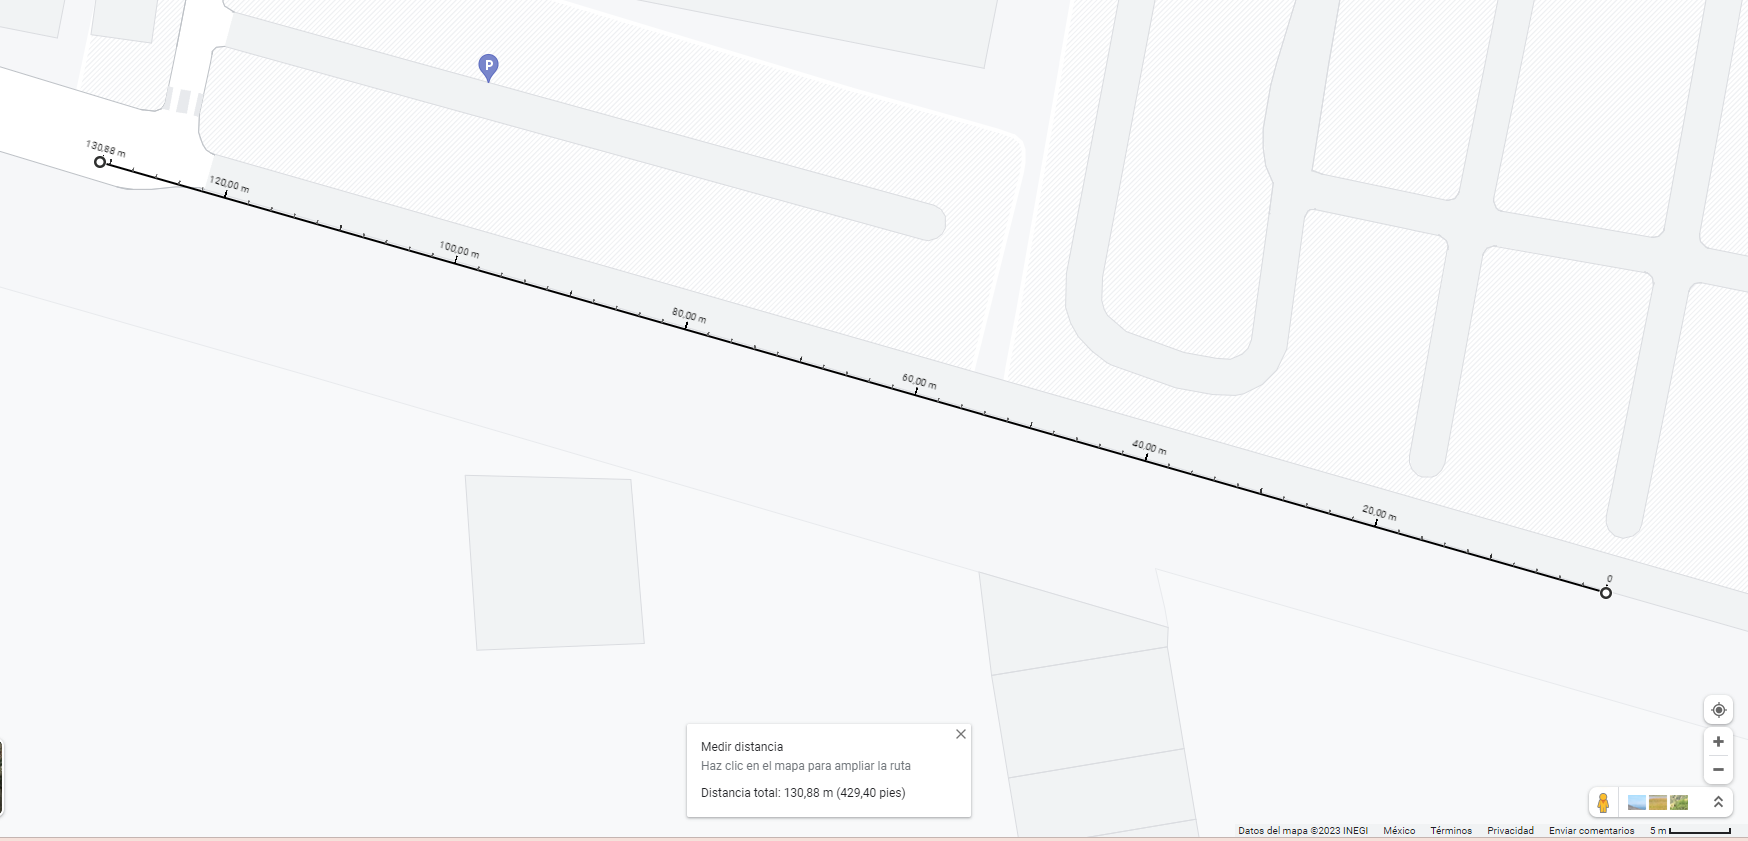
\includegraphics[width=\textwidth]{receiver_test_distance}
			\end{subfigure}
			\caption{Range test.}
			\label{fig:range}
		\end{figure}
	\end{frame}

	\begin{frame}
		\frametitle{Height sensor test}
		\begin{figure}
			\centering
			\begin{subfigure}[b]{0.48\textwidth}
				\centering
				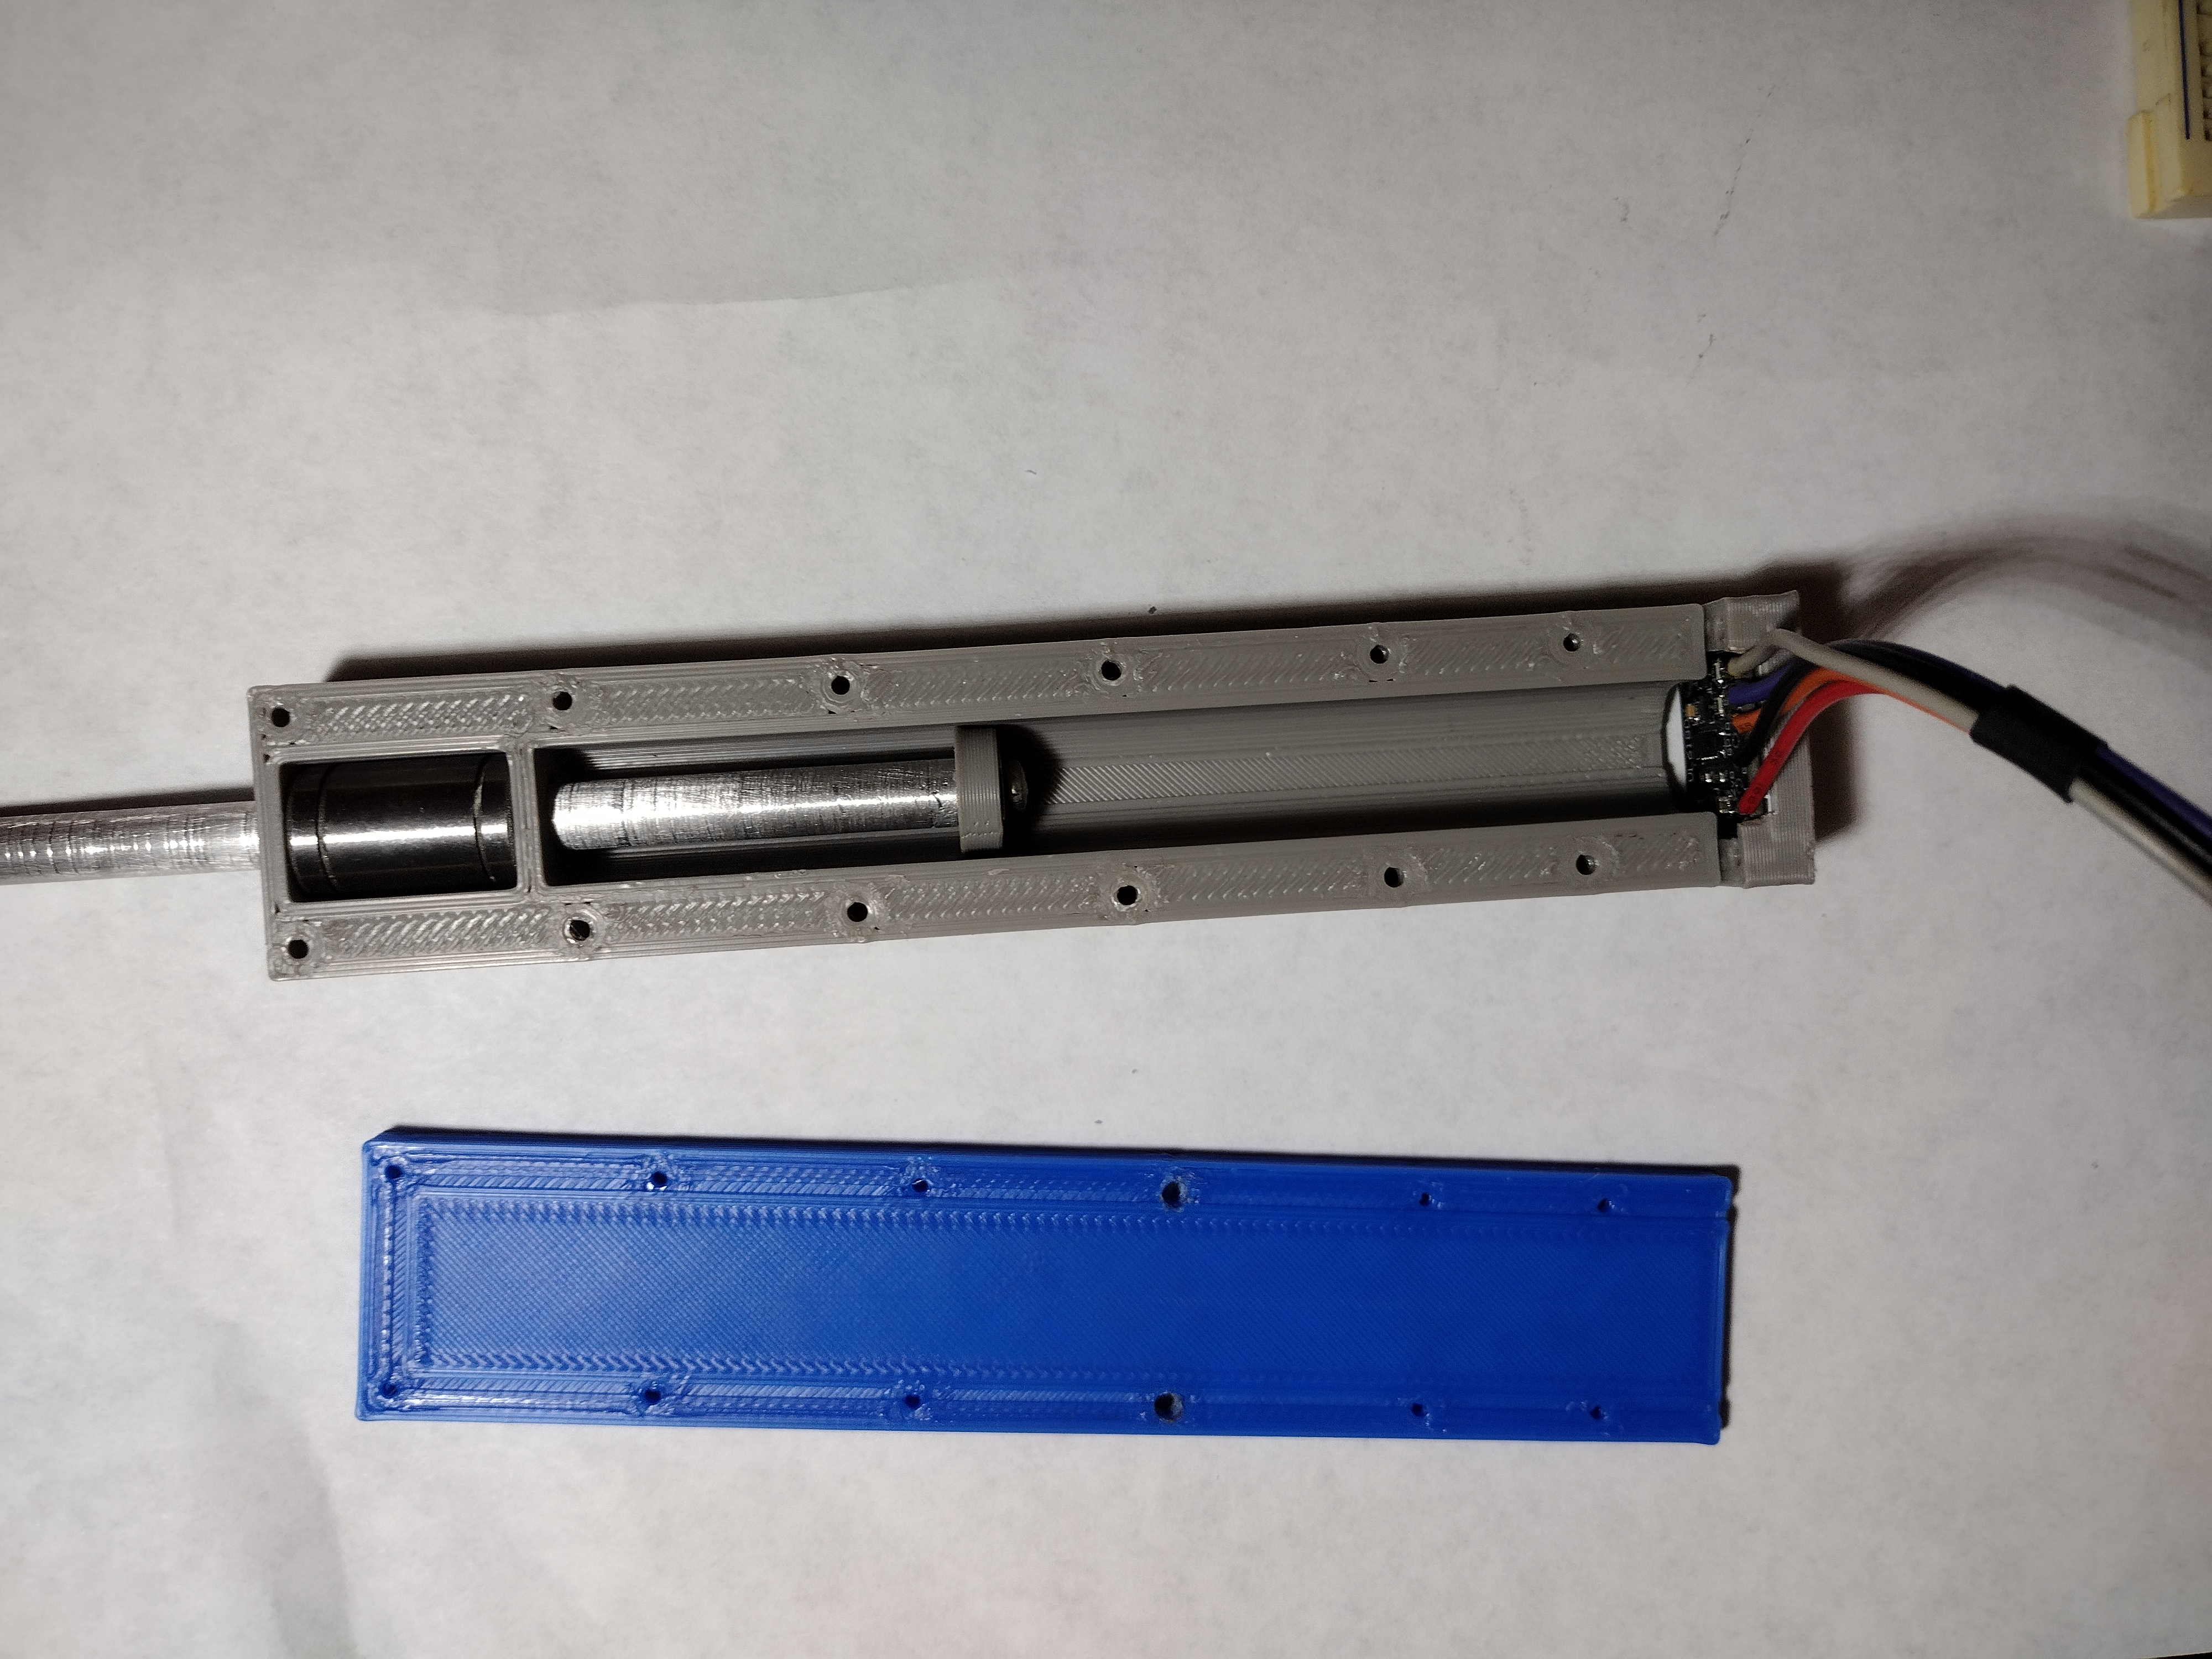
\includegraphics[width=\textwidth]{height_Sensor_1}
			\end{subfigure}
			\hfill
			\begin{subfigure}[b]{0.48\textwidth}
				\centering
				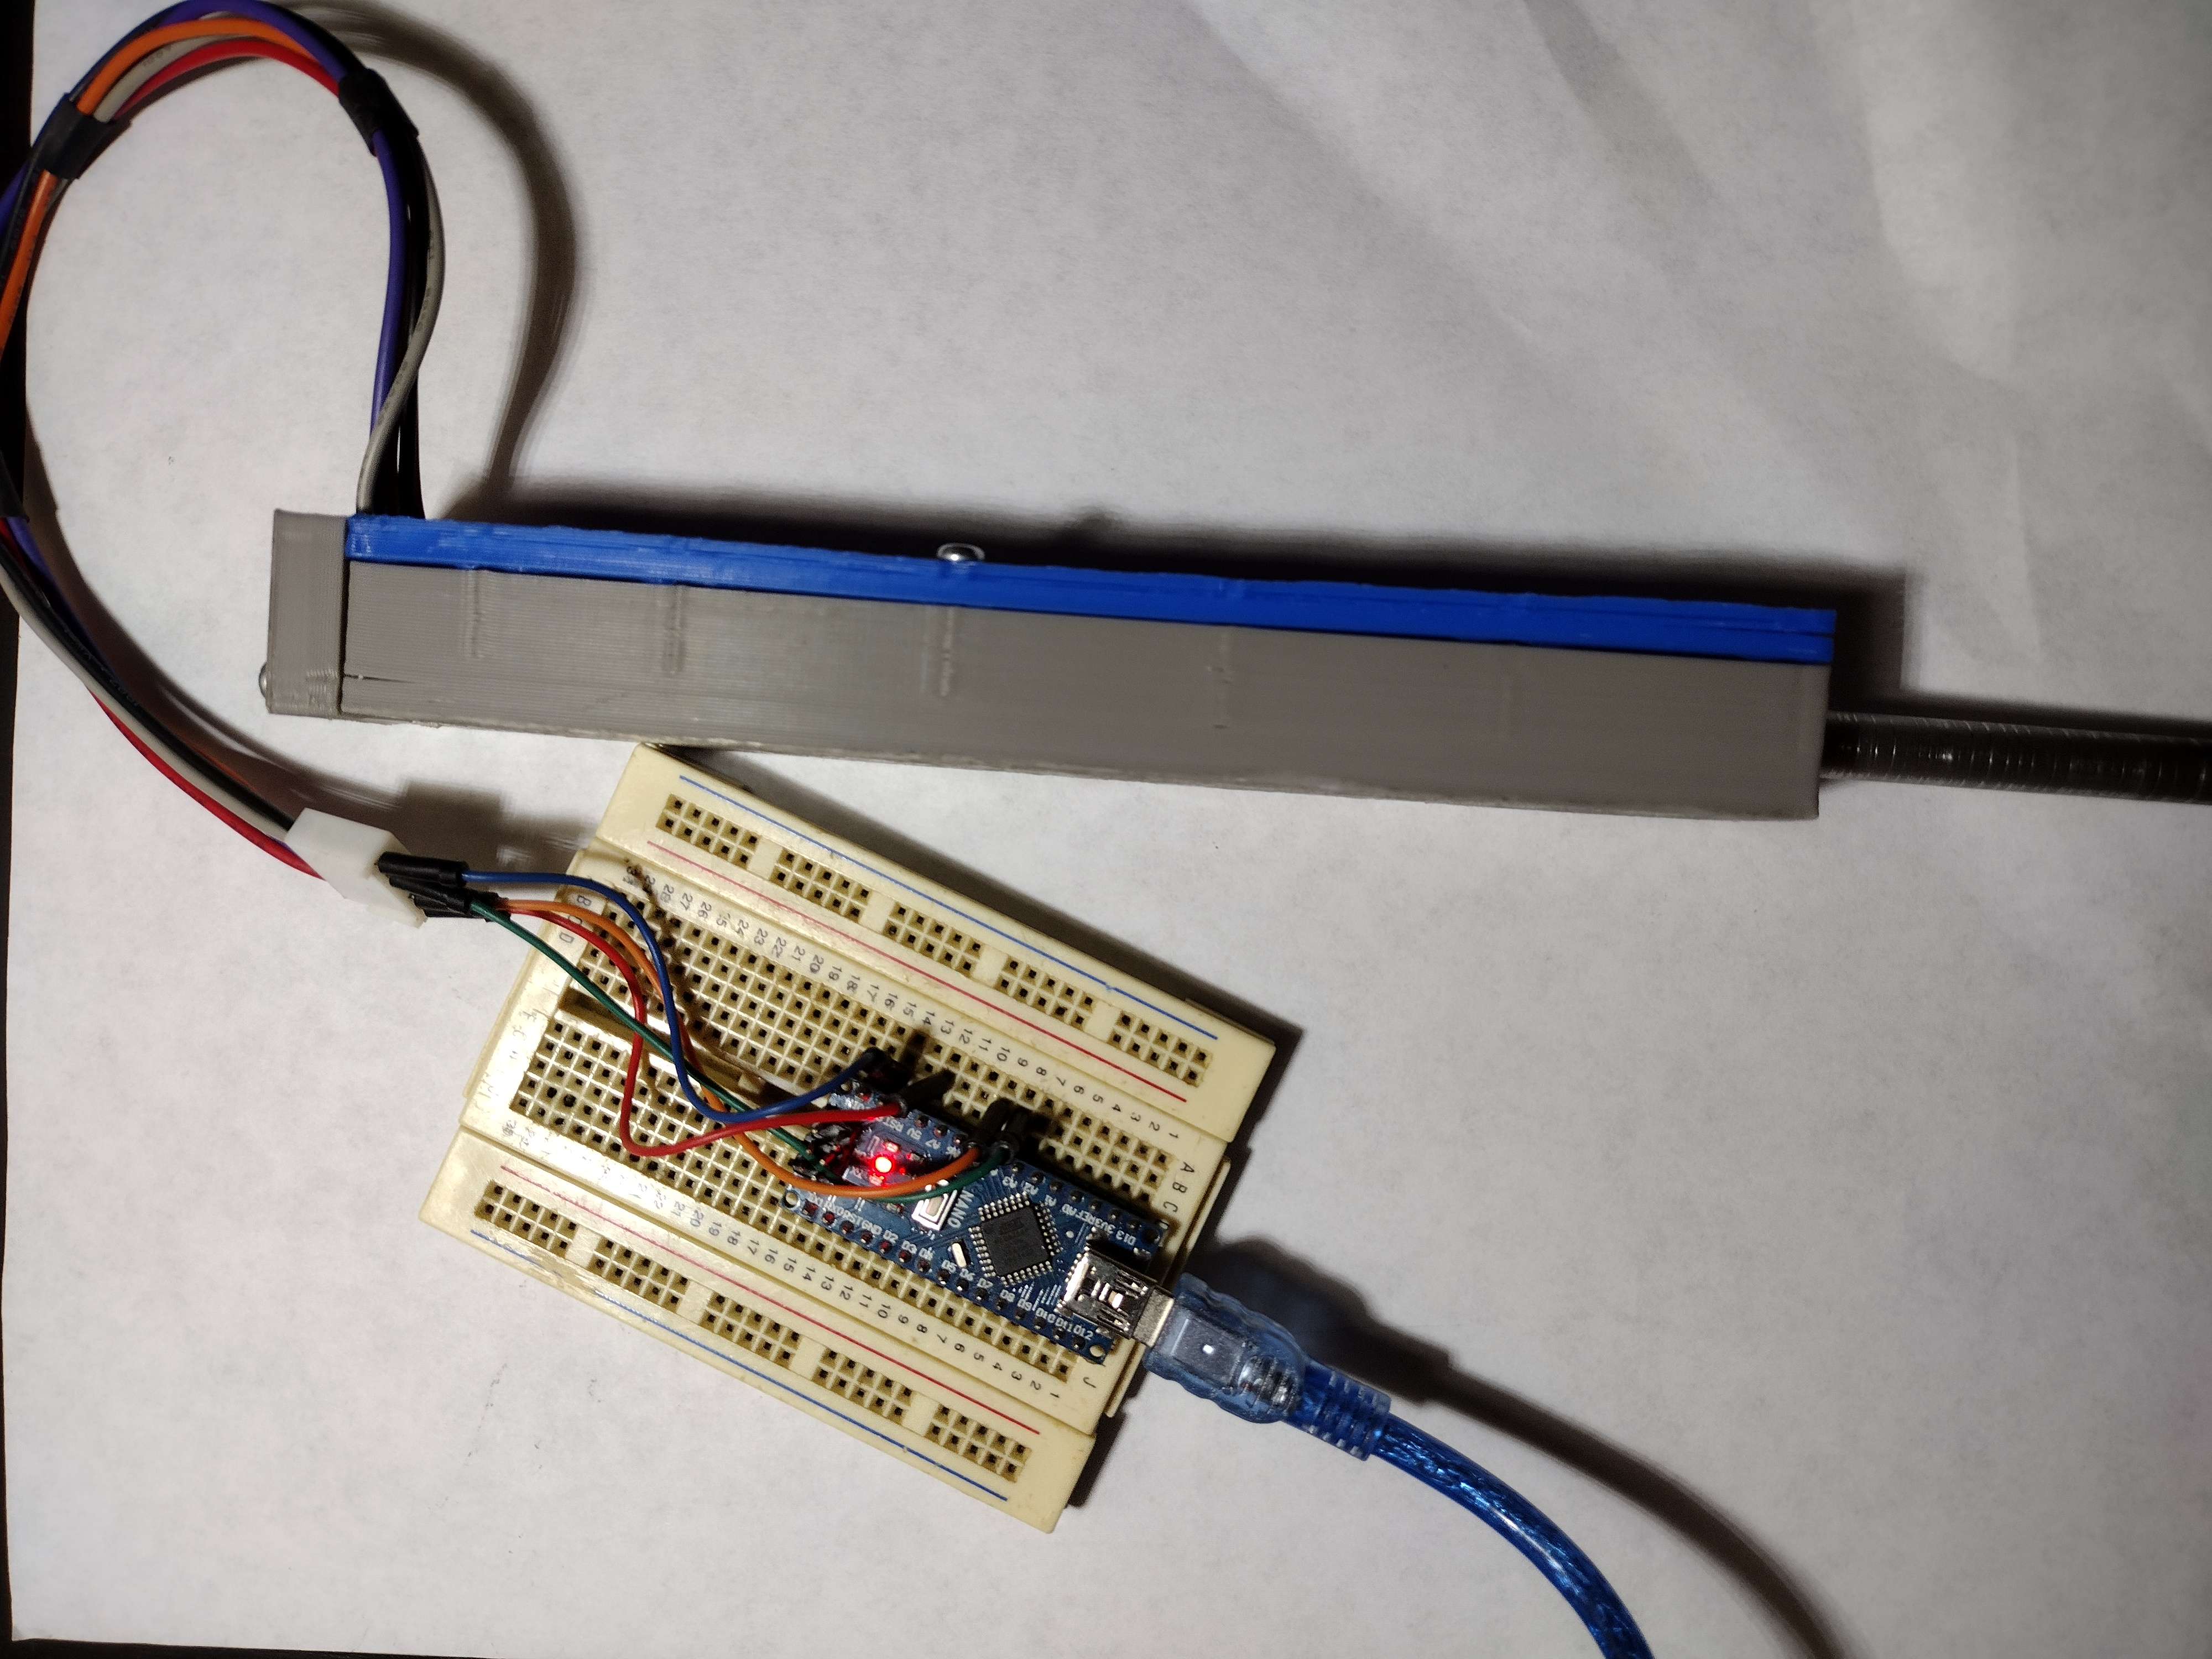
\includegraphics[width=\textwidth]{height_Sensor_2}
			\end{subfigure}
			\caption{Height sensor prototype.}
			\label{fig:height}
		\end{figure}
	\end{frame}


	\begin{frame}
		\frametitle{Interface prototype}
		\begin{figure}
			\centering
			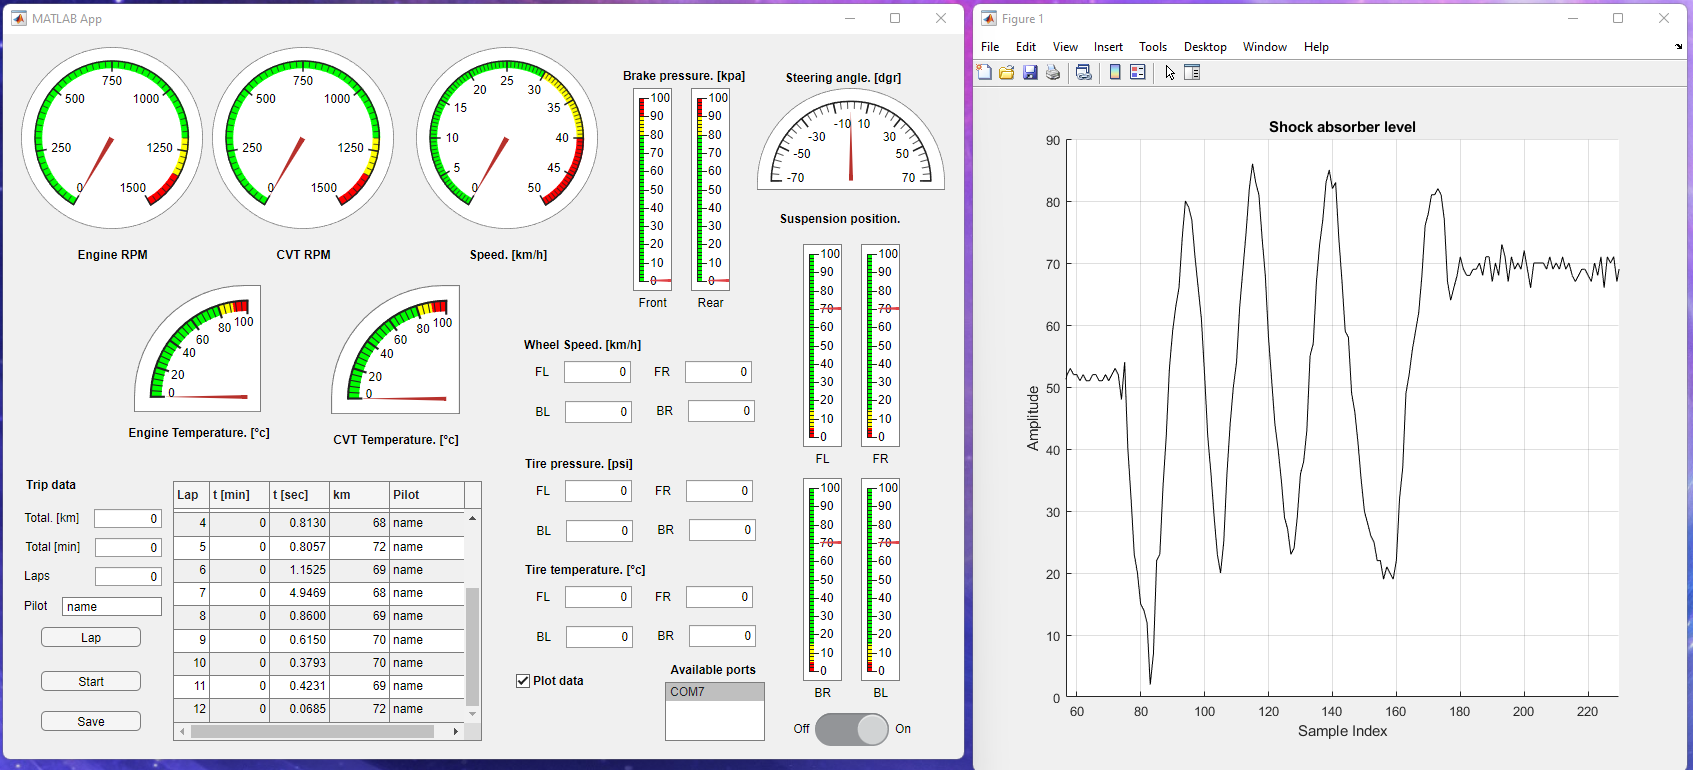
\includegraphics[width=\textwidth]{gui}
			\caption{Test of the GUI.}
			\label{fig:gui}
		\end{figure}
	\end{frame}

	\begin{frame}
		\frametitle{Schematic diagram}
		\begin{figure}
			\centering
			\begin{subfigure}[b]{0.3\textwidth}
				\centering
				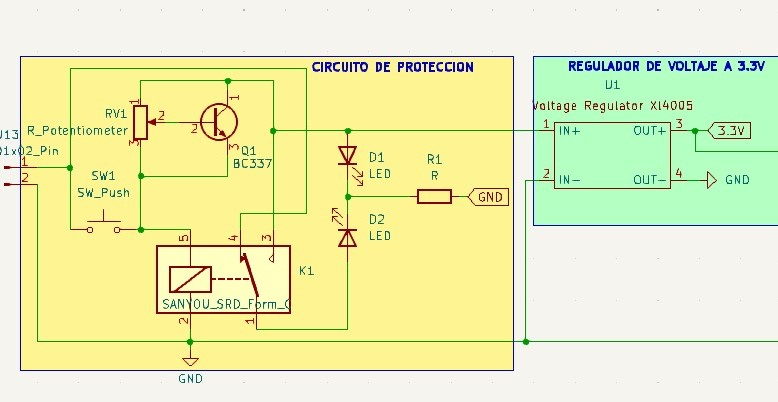
\includegraphics[width=\textwidth]{diagram_1.1}
			\end{subfigure}
			\hfill
			\begin{subfigure}[b]{0.69\textwidth}
				\centering
				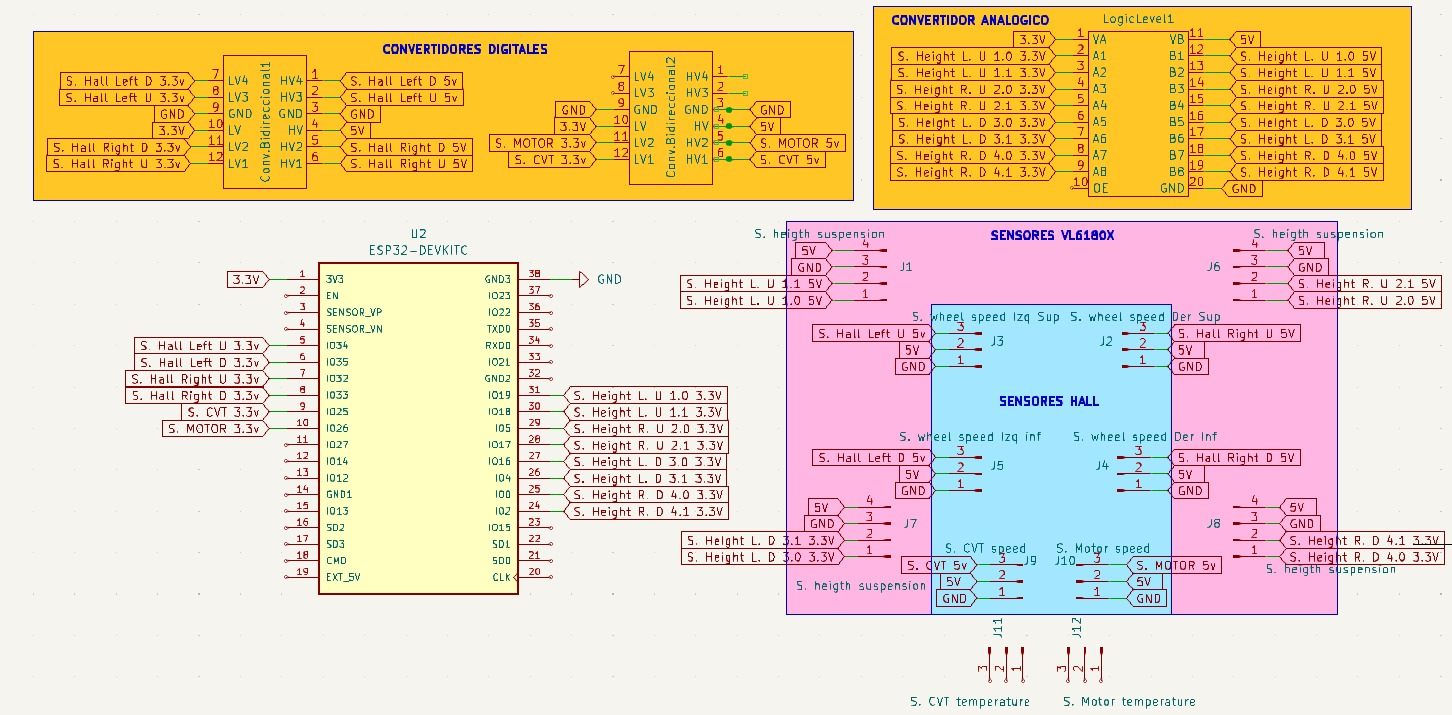
\includegraphics[width=\textwidth]{diagram_2}
			\end{subfigure}
			\caption{Designs of the electronic circuit.}
			\label{fig:}
		\end{figure}
	
	\end{frame}

	\section{Requirements}
	\begin{frame}
	\frametitle{Collaborative work proposals}
	
	\begin{itemize}
		\item We need to manufacture the engine collector and to know the clearance between the engine and the cover of the future design.
		\item We need to know if some teams require the data of another variable.
		
	\end{itemize}

	\end{frame}

	\end{document}

